\section{Simulation}
In this chapter, we empirically test the performance of our proposed and the already existing estimators for \ac{SC} in different \ac{DGP}. Independent of the specific features of the data in terms of pre- and post-treatment period length and the prevailing time series structures, we proceed as follows: We simulate $T_{pre} = T_0 -1$ periods of pre-treatment and $T_{post} = T - (T_0 -1)$ periods of post-treatment data for the single treated unit and the $J$ donor units. Each estimator's main goal is to grasp the consistent patterns before treatment and accurately extend these into the time after treatment. Said differently, the pre-treatment phase depicts the training set of the models and the post-treatment the validation set. To root the simulation framework as close as possible to real-world \ac{SC} applications, we define $T_{pre}$ and $T_{post}$ such that their range is comparable to low-frequency macroeconomic settings, i.e. $T_{pre} \in \left\lbrace 20,50,100\right\rbrace $ and $T_{post} \in \left\lbrace 10,20,30\right\rbrace$. Furthermore, we consider two types of \ac{DGP}, a static factor process and a dynamic \ac{VAR}-process that is inspired by real \ac{GDP} processes of the G20 countries.

\subsection{Static Data Generating Processes}
\subsubsection{Set up}
In their \ac{SC} application of estimating the causal effect of California's proposition 99, \cite{abadie:2010} suppose that the (potential) outcome $Y_{i,t}^{N}$ follows a factor model of the  form 
\begin{equation*}
	Y_{i,t}^{N} = \alpha_t + \theta_t Z_i + \lambda_t \mu_i + \epsilon_{it}.
\end{equation*}
$\alpha_t$ denotes an unknown panel-invariant intercept, $Z_i$ is a vector of observed panel-specific covariates, $\theta_t$ is a vector of unknown parameters, $\lambda_t$ is a vector of unknown common factors and $\mu_i$ are panel-specific unknown factor loadings. The unobserved shocks $\epsilon_{it}$ have zero mean at the panel level. 
For this specific setting, \cite{abadie:2010} show that "[...] the bias of the SC-estimator can be bounded by a function that goes to zero as the number of pre-treatment periods increases." Further the number of donor units has to be fixed. The fact, that $\alpha_t$ is panel-invariant seems minor at first glance. However, as the \ac{SC}-estimator does neither contain an intercept nor does it allow for extrapolation outside the convex hull of the donor pool, the unbiasedness of the estimator directly depends on the distribution of the intercepts. In a slightly more realistic data-generating scenario, the intercepts do not follow a degenerate point distribution with $P(X = 0) = 1$ but are drawn from a symmetric distribution centered around the origin like the standard normal. 

\cite{ferman:2021} considers a de-meaned scenario without additional covariates. In our static simulation, we follow the basic set-up of Ferman and generate data according to a similar factor model. However, we consider it more realistic to add a time-invariant and panel-specific intercept to the (potential) outcome instead of analyzing a de-meanded \ac{DGP}. Our representation of the counterfactuals therefore boils down to 
\begin{equation*}
	Y_{i,t}^{N} = \alpha_i + \lambda_t \mu_i + \epsilon_{it}.
\end{equation*}
In this simplified setting, the counterfactual is given by the composition of the unknown panel-specific factor loadings $\mu_i$ and the $F$ unknown common factors $\lambda_t = (\lambda_{1,t}, ..., \lambda_{F,t})$ plus intercept $\alpha_i$ and idiosyncratic shocks $\epsilon_{it}$. For the sake of simplicity, Ferman considers a scenario with only two common factors, $\lambda_{1,t}$ and $\lambda_{2,t}$. We proceed analogously and generate data such that the (potential) outcome of the treated unit and the first half of the donor pool load exclusively with loading one on the first factor, the remaining donors load exclusively with loading one on the second factor. Therefore $\mu_i$ is a $(2 \times 1)$-vector with the first (second) entry being one and the second (first) entry being zero for the first (second) half of the donor pool. Further, the random variables $\alpha_i, \lambda_{1,t}, \lambda_{2,t}$ and $\epsilon_{it}$ are realizations of \ac{iid} standard normal distributions $\mathcal{N}(0,1)$. The following figure exemplifies the functionality of the \ac{DGP} with $T_{pre} = 20$ and $T_{post} = 10$ and a constant treatment effect of $\delta_{0,t} = 10$ for $t > T_0$.\footnote{In this example, the series $j = 0$ is treated at $T_0 = 20$, while the impact of the treatment becomes noticeable one time period later, starting from $t > T_0$. Note that the actual treatment effect is irrelevant for our investigation as it is empirically observable.}  
\begin{figure}[H]
	\centering
	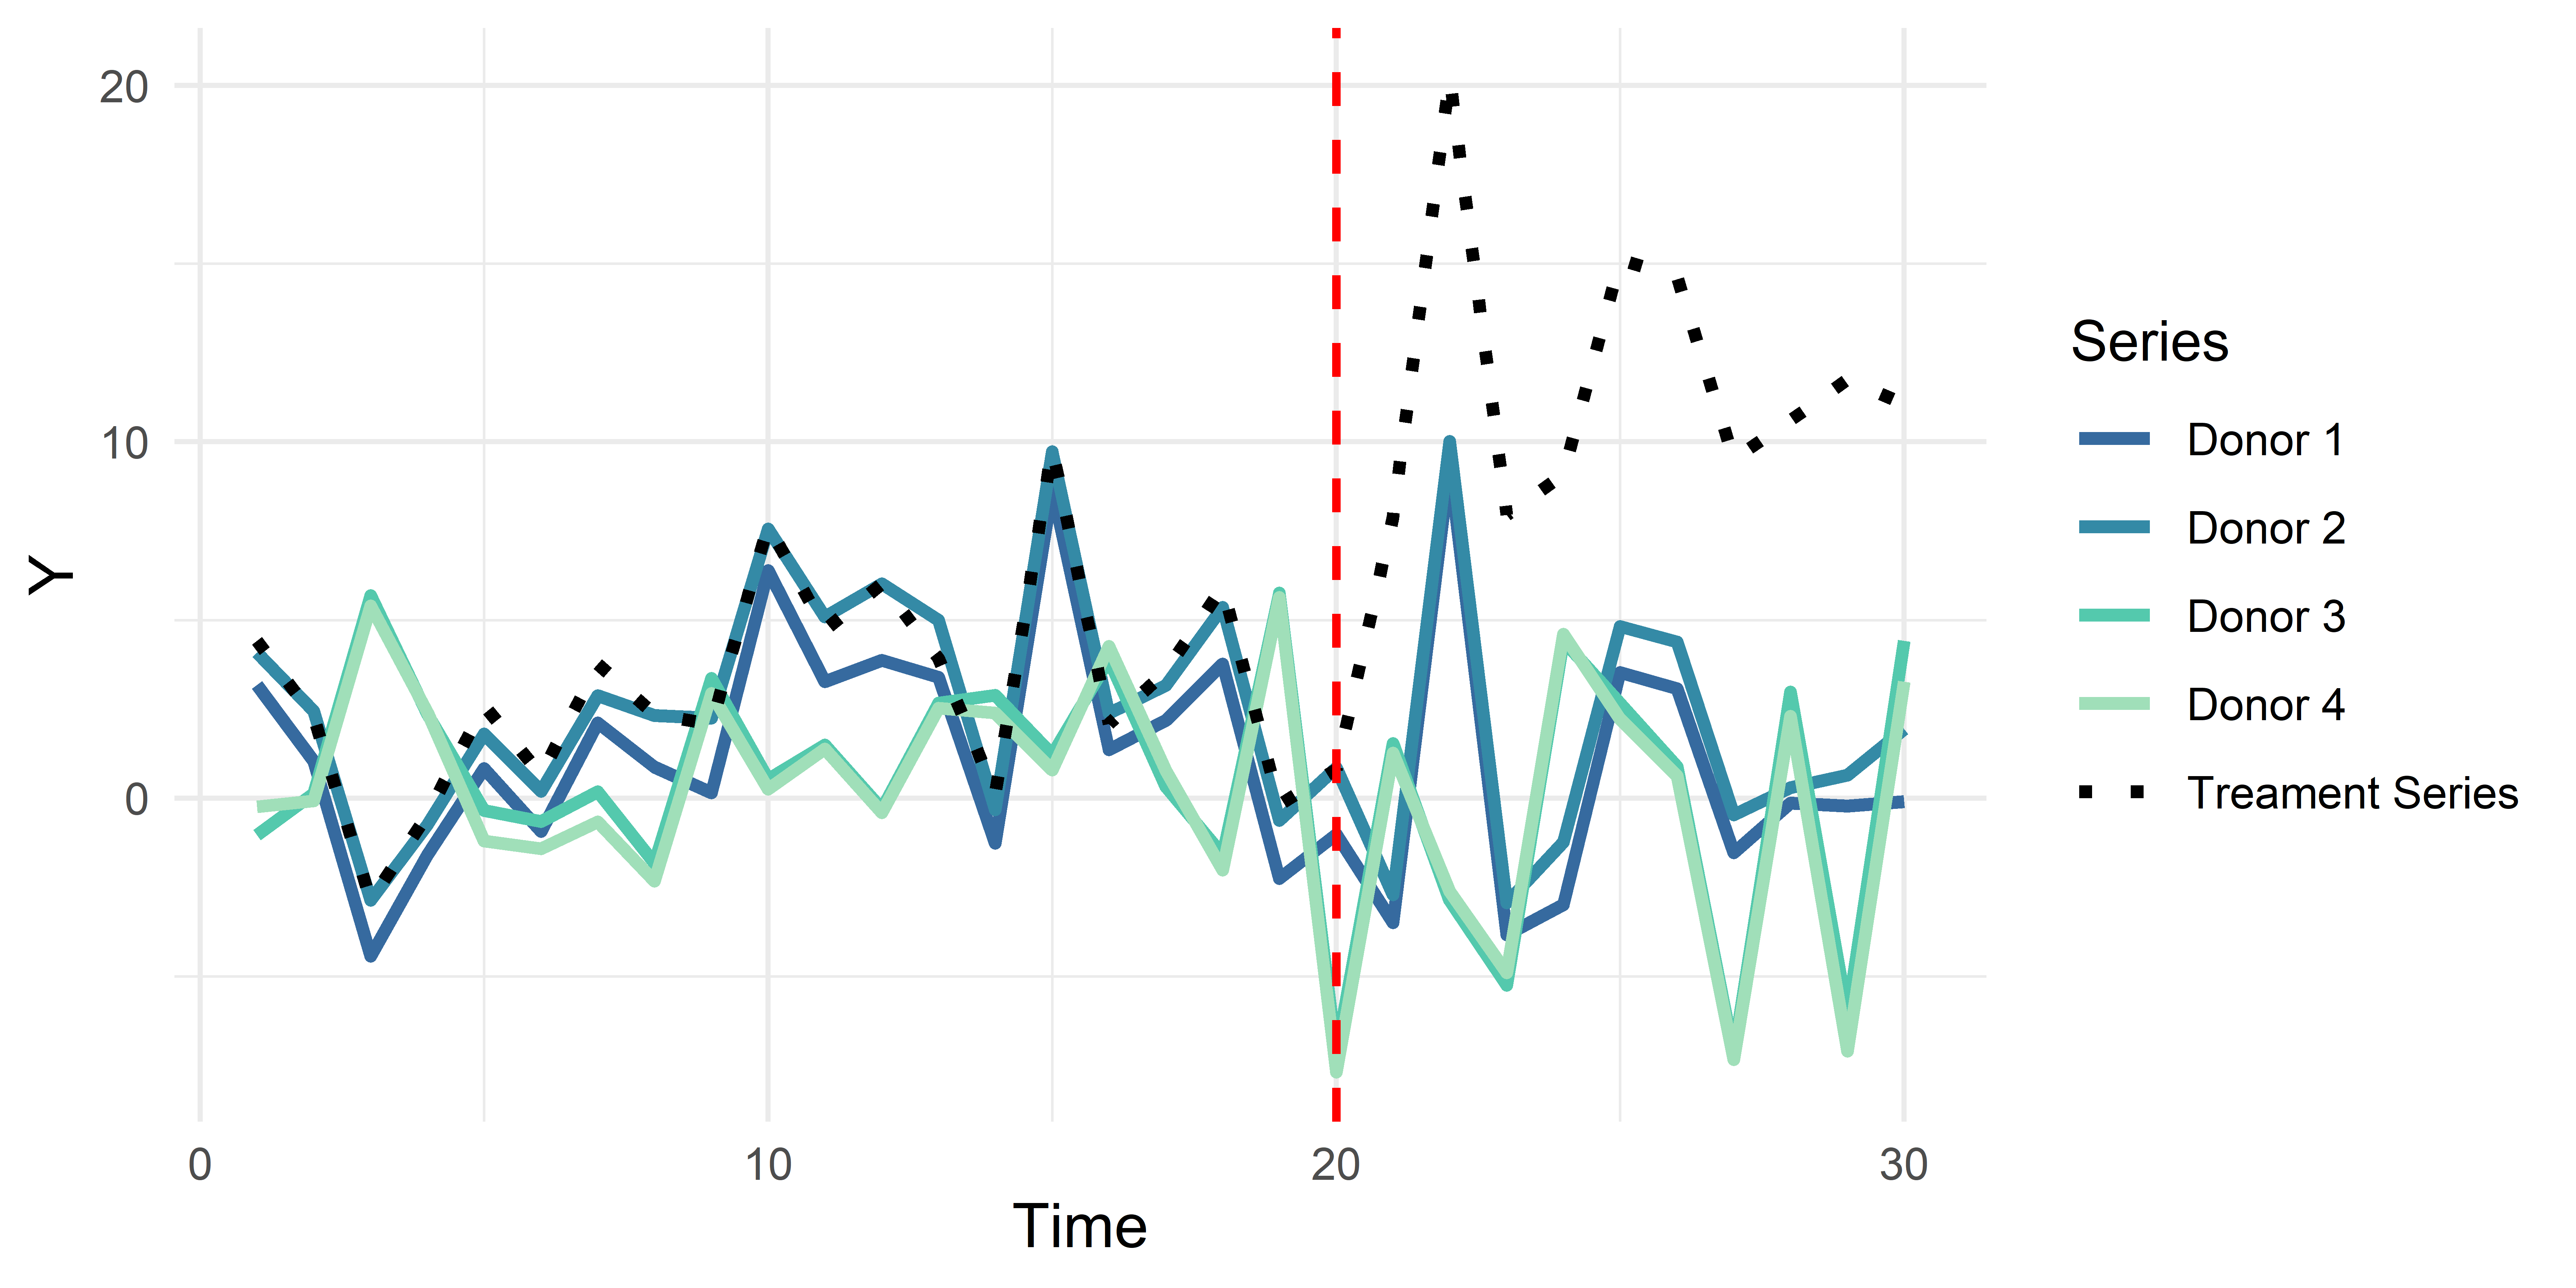
\includegraphics[scale=.9]{F02}
	\caption{Example Factor-\ac{DGP}}
	\label{F_02}
\end{figure}
To make the factor structure more tangible, we scaled the factor variances by $10^1$ and the error variance by $10^{-1}$. The generated data exhibits a clearly observable factor structure: The treatment unit and the first half of the donors (Donor 1 and 2) as well as the second half of the donors (Donor 3 and 4) share a common factor. Thus, the objective of each employed method is to recover the true factor structure, i. e. irrelevant of the size of donor pool to weight only the first $\frac{J}{2}$ donors positively. Further, we see that each series possesses an own intercept. Yet in this specific example only, the intercept variation is dominated by the factor variation due to the scaling of the variances.

\subsubsection{Employed Models}
For the static factor \ac{DGP}, we employ five models: 

SC: The first model is the ordinary \ac{SC} method without additional covariates. Therefore, this method is equivalent to a restricted \ac{OLS} regression that regresses the treatment series on the donors series given the constraint of no intercept and non-negative coefficients that sum up to one. The belief for this model is that the untuneable restrictions prevent it from overfitting the pre-treatment data but that this inelasticity comes at the costs of a reduced predictive performance.

OLS: The second model is a usual least squares regression that regresses the treatment series on the donor series. The belief for this model is that it starts overfitting the pre-treatment data as $J$ grows large as it exhibits no regularization opportunities. Further for $J > T_0$, it is unable to provide any prediction or forecast.

NET: The third model we consider is the aforementioned elastic net as proposed by \cite{doudchenko:2016} in the context of \ac{SC}. Due to its flexible hyperparameters tuned via pre-treatment \ac{CV}, we expect this model to perform reasonable well over the entire observation window (pre- and post-treatment). For the sake of simplicity and due to the short training periods, we perform a simple 3-fold \ac{CV} and rely on highly efficient R-implementation of the elastic net "glmnet" of \cite{friedman:2010}. In the conceptual introduction of the elastic net, we stressed the potential drawback of having no closed form solution. As a consequence, we assume the model to perform worse in small samples.

REGSC: The fourth model under consideration is our proposed regularized synthetic control model which can be interpreted as a mixture of the elastic net and the original \ac{SC} estimator. It is comparable to the elastic net insofar that it simply substitutes the Lasso-shrinkage by the inverse-Ridge-shrinkage. This substitution is motivated by the \ac{SC}-specificity of having percent-like coefficients. Thus, we expect the model to perform well especially in settings that are comparable to the original \ac{SC} setting like the static factor \ac{DGP}. Its closed form solution and the increased flexibility caused by the tuneable hyperparameters make us confident that the model performs equally well in small and in large samples as well as in the pre- and the post-treatment period. To reduce computation time, the optimal hyperparameters are obtained by 2-fold \ac{CV} in a two-step random grid-search procedure. Random hyperparameter grid search has proven to be more efficient than manual grid search both theoretically and empirically. See for instance \cite{bergstra:2012} for a careful discussion of hyperparameter optimization. Specifically, we start by spaning a large $50 \times 50$ grid with $\lambda_1$ ranging from 5 to 3,125 and $\lambda_2$ ranging from 10 to $10^7$ and randomly select 400 out of the 2,500 $\lambda_1$-$\lambda_2$-combinations.\footnote{In sensitivity checks, we found that wider intervals did not change the location of the potential optimum. However, the optimal range will always be case-specific.} In the first step of the procedure, we identify the optimal hyperparameter combination of the initialized grid by applying 2-fold \ac{CV}. Based on the result of the first step, we enclose the potential optimum in the second step by sequentially holding the first and the second hyperparameter fixed while increasing and decreasing the remaining hyperparameter on a coarser grid. Note that a more efficient \ac{CV}-procedure could potentially improve the \ac{REGSC}-method.

FACTOR: The data of this process is generated such that the common factors and the idiosyncratic component are uncorrelated and that the idiosyncratic errors are mutually uncorrelated. Thus, the static factor model which estimates the common factors as linear function of the donors is the most natural candidate model. The \ac{PC} estimator is a popular estimator for the factor model. It is employed as follows: In the pre-treatment period, we obtain the predictions by regressing the treatment series on the "latent" factors. As we implemented a two-factor structure, the factors are computed by multiplying the first two eigenvalues of the covariates matrix of the donors with the matrix of the covariates of the donors. The forecasts for the post-treatment period are obtained by multiplying the factor structure of the post-treatment period with the regression coefficients of the pre-treatment regression. As this model directly build upon the \ac{DGP}, it is our benchmark-model and we expect it to perform best among all candidates.\textcolor{magenta}{\textbf{(@ Jörg Breitung: why no overfitting?)}} 

For each of the 9 combinations of pre- and post-treatment period length and the 6 investigated donor group sizes, we simulated 1,000 static factor processes as described above.\footnote{Remember that $T_{pre} \in \left\lbrace 20,50,100\right\rbrace $, $T_{post} \in \left\lbrace 10,20,30\right\rbrace$ and $J \in \left\lbrace 5,10,15,20,25,30\right\rbrace$.} This extensive simulation provides us with a total of 54,000 processes that are analyzed with respect to the following precision and dispersion metrics in the post-treatment period:
\begin{itemize}
	\item \ac{RMSFE}: The \ac{RMSFE} is the central loss function of our analysis. It has the following form:
	$$RMSFE(m) = \left(\frac{1}{T - T_0} \sum_{t = T_0}^{T} \left( y_{0,t} - \delta_{0,t} - \widehat{y}_{0,t}(m)\right) ^2 \right)^{1/2},$$
	
	where $m$ present one of the five employed models. Due to its quadratic nature, it is not only a reasonable approximation to realistic loss structures but also mathematically convenient \cite{diebold:2017}. 
	\item Bias: The \ac{RMSFE} is unable to distinguish between over- and underestimation as deviations from the true target quantity are squared. The bias is directly related to the $RMSE$ but provides a more detailed measure in terms of error location. It is computed as follows:
	$$BIAS_m = \frac{1}{T - T_0} \sum_{t = T_0}^{T} \widehat{y}_m - (y_{0,t} - \delta_{0,t}),$$
	such that negative values indicate under- and positive values overestimation. This precision metric is especially important when analyzing intercept-free models as these models will exhibits a bias whenever the treatment intercept falls outside the donor intercepts. 
	\item \ac{MZ} regression: The \ac{MZ} regression tests the forecast optimality in a different and more holistic way by regressing the true value on its predicted value in the post-treatment period: 
	$$y_{0,t} = \beta_0 + \beta_1 \widehat{y}_{0,t} \text{ for } t \geq T- T_0.$$
	If the forecast is optimal, we expect to observe that $(\beta_0, \beta_1) = (0,1)$, an hypothesis that is directly testable by a simple F-test. In comparison to the RMSE and to the bias, this approach superior because we can report average, simulation-overarching quantities without wiping out crucial details like negative and positive biases. In our simulation, we report the share of iterations in which the F-test was unable to reject the joint hypothesis of $(\beta_0, \beta_1) = (0,1)$ at the conventional significance level of 5\%. The closer this share to unity, the closer the specific forecast to the optimal quantity. Due to varying sample sizes, however, those shares are only interpretable at the within-simulation level.
	
	\item Variance: To observe the variability of the employed models, we also compute their intra-simulation variances as
	$$VAR(m) = \frac{1}{T - T_0} \sum_{t = T_0}^{T} \left( y_{0,t} - \delta_{0,t} - \widehat{y}_{0,t}(m)\right) ^2 $$

\end{itemize}
\subsubsection{Results}
The full simulation results in table format can be found in the appendix \ref{Static simulation} where we group the tables at the level of the six analyzed donor quantities. Here, we present the central tendencies of the simulation. To do so, consider the following figure that plots the average \ac{RMSFE} of the models against the size of the donor pool for $T_{pre} = 50$ and $T_{post} \in \left\lbrace 10,20,30\right\rbrace$.\footnote{As we found that the length of the post-treatment period is less important to explain the models performance, we pool the three elements of $T_{post}$ at this point. The depicted means are thus computed on the basis of 3,000 iterations each.} 

%\textcolor{magenta}{\textbf{(Important to distinguish different intercept cases: If the intercept of the treated series falls outside the donor-intercepts, SC exhibits a bias as it does not allow for a panel-specific constant.)}} 


\begin{figure}[H]
	\centering
	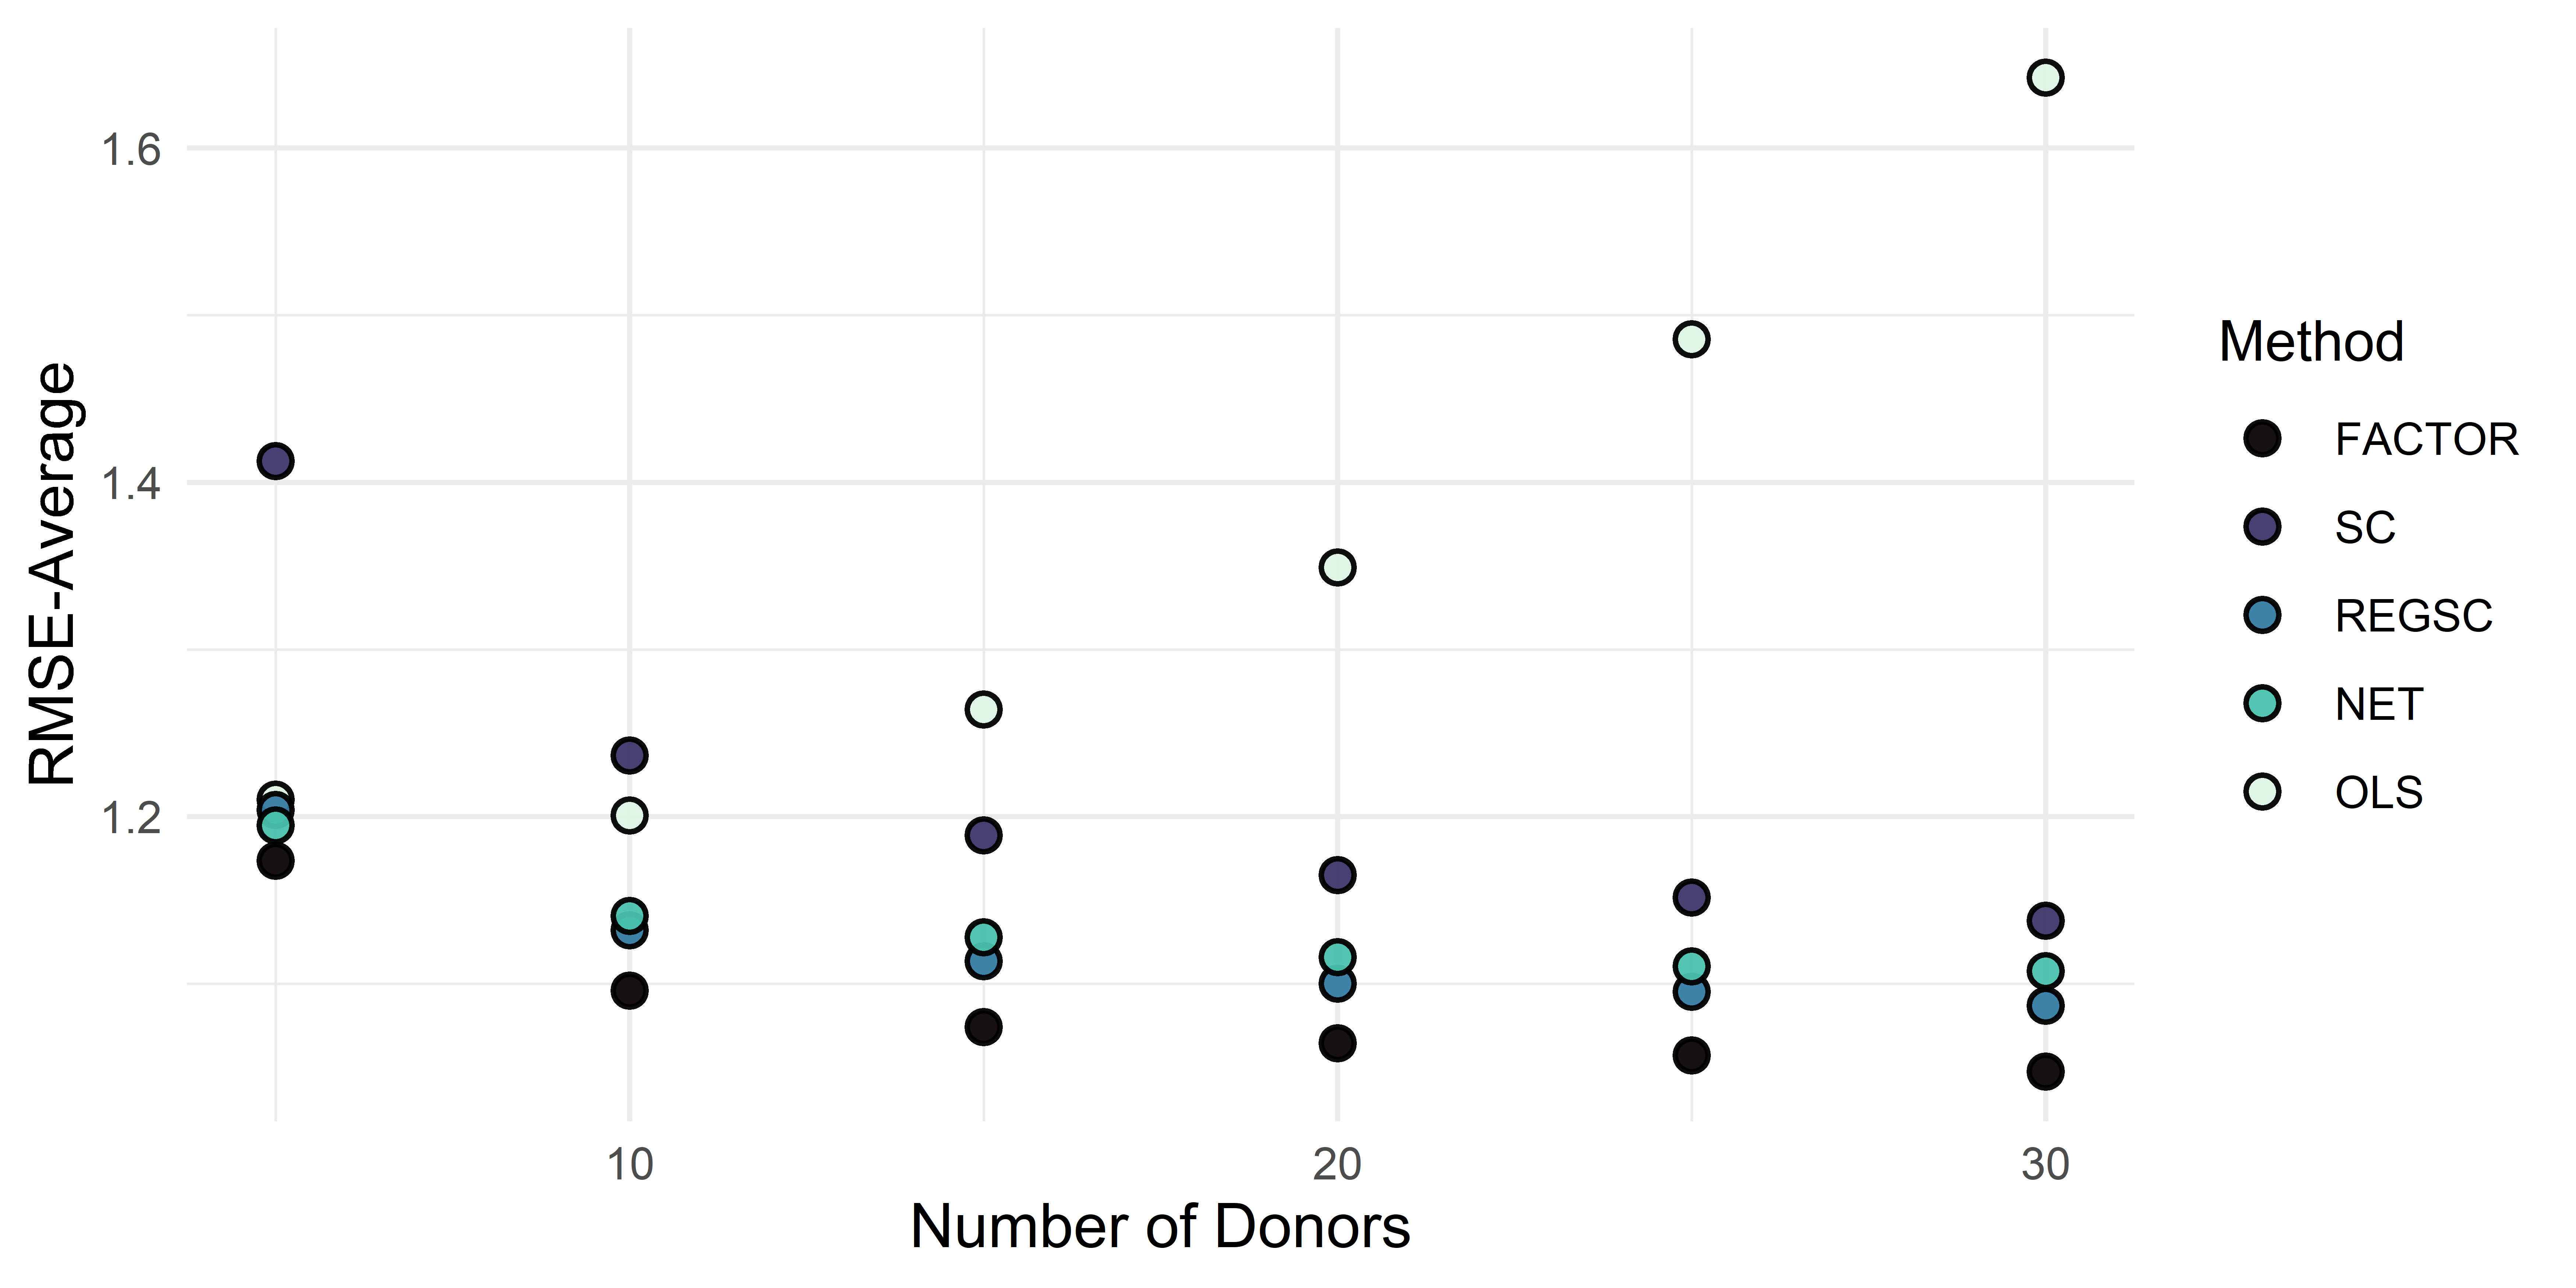
\includegraphics[scale=.9]{F07}
	\caption{Simulation Performance for $T_{pre} = 50$ and $T_{post} \in \left\lbrace 10,20,30\right\rbrace$}
	\label{F_07}
\end{figure}

Five observations stand out: First, as expected, the unrestricted \ac{OLS} regression starts to overfit the pre-treatment data quite fast indicated by a \ac{RMSFE} that starts to increase from $J = 10$ onward. This tendency consistently aggravates as $J$ approaches $T_{pre}$. Second, the remaining models seem to successfully distinguish between systematic pre-treatment patterns and noise as their forecasts improve with increasing $J$. Third, in terms of relative performance, for obvious reasons the factor models extrapolates the process best into the post-treatment period. Fourth, the elastic net and our proposed \ac{REGSC} estimator perform comparable with slight comparative advantages toward the latter. These differences are more pronounced in small samples which can be interpreted as a sign of the small sample robustness of the closed form solution. Last but not least, the \ac{SC} estimator, though being able to not overfit the training data, consistently performs worse than the elastic net and the \ac{REGSC} estimator. 

It has been stressed that the \ac{RMSFE} should not be the only precision metric when evaluating  forecast performances as it is unable to detect over- and underestimation. On the other hand, the bias, though being able to flag iteration-specific over- and underestimations, can indicate spurious optimality when it is aggregated.\footnote{Consider for instance a model that forecasts $\left\lbrace -1,1\right\rbrace $, each in 50\% of the cases for a quantity whose optimal forecast is 0 in 100\% of the cases. This model is far from optimal but the mean bias is 0. } To solve this problem, we can either consider the bias-distributions or rely on the p-values of the \ac{MZ}-regressions. Let us first focus on the bias-distributions: Above, we argued, that intercept-free models like the \ac{SC}-method will exhibit a positive (negative) bias whenever the mean of the treatment-series exceeds (falls below) the means of the donor series. In our simulation, the intercepts of the series are \ac{iid} realizations of standard normal distributions. Therefore, the probability that the mean of the treatment series falls below (exceeds) all donor means equals $\frac{1}{J+1}$.\footnote{For each donor quantity $J$, there are $(J+1)!$ total orderings. In $\frac{(J+1)!}{J+1}$ of the cases, the intercept of the treatment series is the most extreme. This translate to a probability of $\frac{1}{J+1}$. } \textcolor{magenta}{\textbf{(@Jörg Breitung: stimmt das? Die Simulationsdaten sprechen dafür)}} In the following figure, we extracted the iterations for which the treatment intercept was the most extreme, grouped these observations according to minimum/ maximum and plotted the post-treatment bias density for the \ac{SC} and the \ac{REGSC} model. 
\begin{figure}[H]
	\centering
	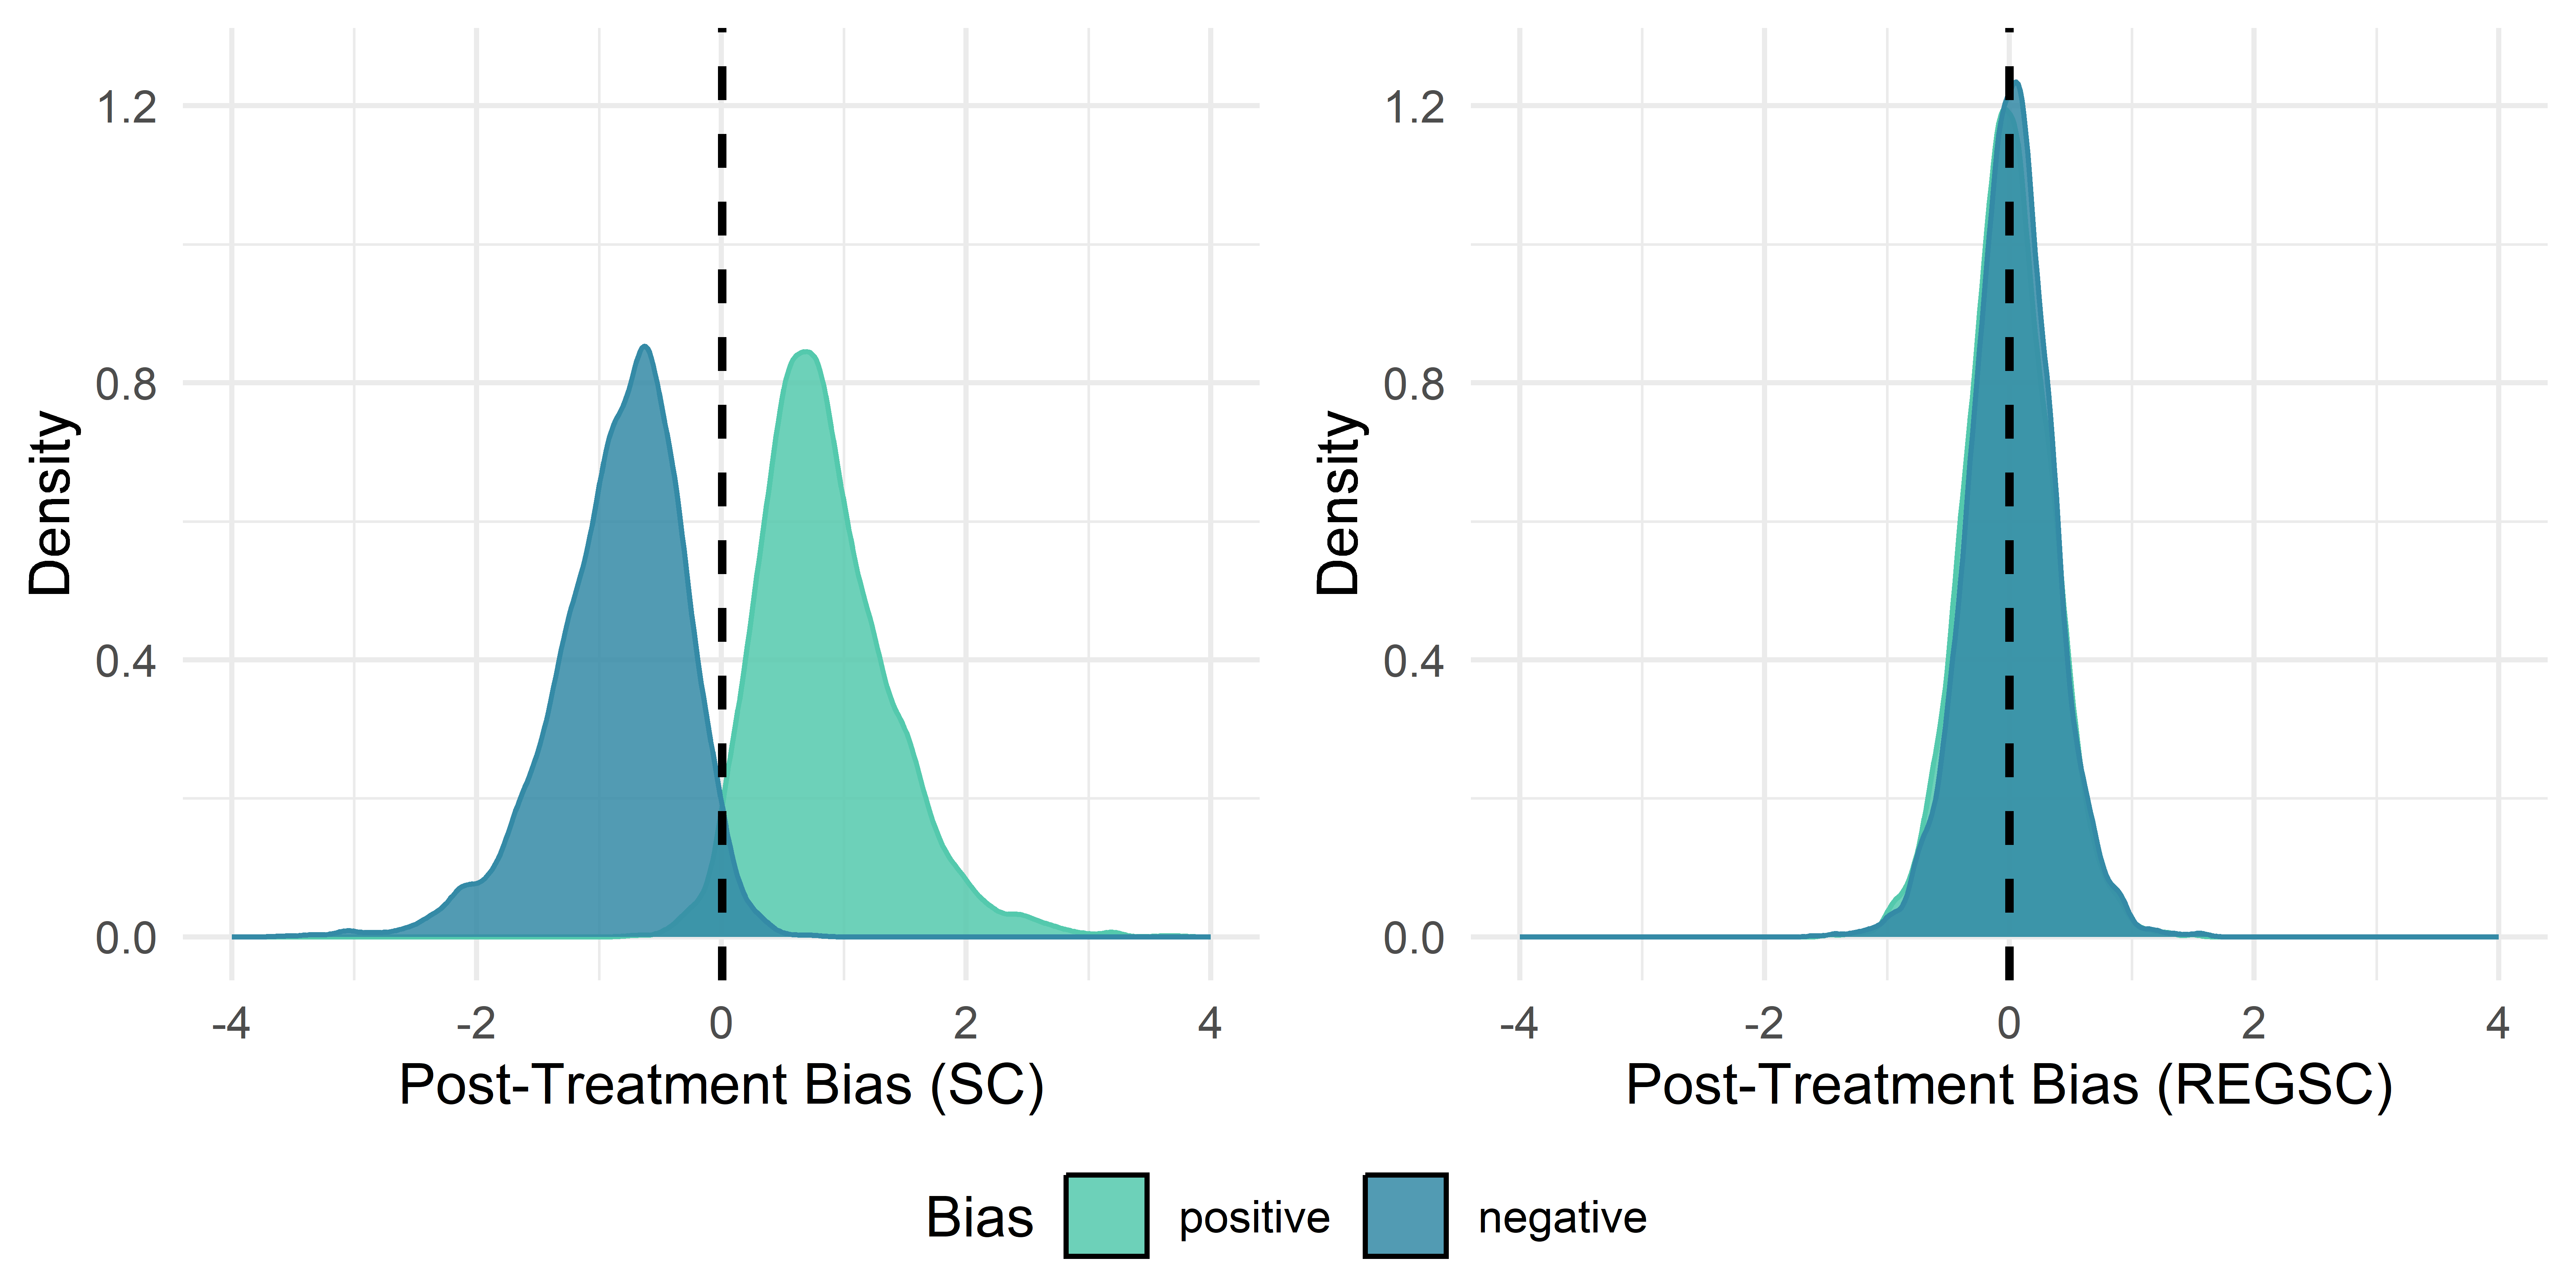
\includegraphics[scale=.9]{F11}
	\caption{Bias-distribution for the SC and the REGSC model}
	\label{F_09}
\end{figure}

The aforementioned problem of the bias becomes immediately apparent: Though both estimator have an average bias that is close to 0, the \ac{SC} method exhibits severe positive/ negative biases if the 
treatment intercept falls outside the convex hull of the donors intercepts. In contrast, the \ac{REGSC} model as well as the remaining models that include an intercepts do not face this issue. 

\newpage
\begin{table}[H]
	\centering
	\noindent
	\caption{Static simulation: Post-treat. share of iterations with MZ-p-value > 0.05}
	\scalebox{1}{
		\begin{tabular}{c c | C{1.5cm} | C{1.5cm} | C{1.5cm} | C{1.5cm} | C{1.5cm} | C{1.5cm} }
			\toprule[1.5pt]
			\multicolumn{1}{c}{$\boldsymbol{T_0}$} & \multicolumn{1}{c}{\textbf{Donors}}& \multicolumn{1}{c}{\textbf{SC}} & \multicolumn{1}{c}{\textbf{OLS}} & \multicolumn{1}{c}{\textbf{REGSC}}& \multicolumn{1}{c}{\textbf{NET}}& \multicolumn{1}{c}{\textbf{FACTOR}} & \multicolumn{1}{c}{\textbf{2nd best}}\\
			\cmidrule(lr){1-8}
			20&5&0.5650&0.6617&0.7413&0.7648&0.8143&NET\\
			20&10&0.6897&0.3777&0.7577&0.7479&0.8050&REGSC\\
			20&15&0.7343&0.1153&0.7517&0.7486&0.8190&REGSC\\
			20&20&0.7600&NA&0.7380&0.7193&0.7993&SC\\
			20&25&NA&NA&0.7427&0.7420&0.7987&REGSC\\
			20&30&NA&NA&0.7433&0.7475&0.8227&NET\\
			\cmidrule(lr){1-8}
			50&5&0.5857&0.8707&0.8677&0.8820&0.8947&NET\\
			50&10&0.7503&0.8237&0.8787&0.8783&0.8940&REGSC\\
			50&15&0.8067&0.7123&0.8703&0.8680&0.8923&REGSC\\
			50&20&0.8103&0.6007&0.8757&0.8717&0.8910&REGSC\\
			50&25&0.8423&0.4333&0.8803&0.8750&0.8920&REGSC\\
			50&30&0.8510&0.3023&0.8680&0.8667&0.8923&REGSC\\
			\cmidrule(lr){1-8}
			100&5&0.6200&0.9100&0.9057&0.9150&0.9193&NET\\
			100&10&0.7757&0.9120&0.9207&0.9277&0.9277&NET\\
			100&15&0.8030&0.8743&0.9140&0.9067&0.9183&REGSC\\
			100&20&0.8430&0.8480&0.9180&0.9157&0.9260&REGSC\\
			100&25&0.8540&0.8097&0.9167&0.9117&0.9247&REGSC\\
			100&30&0.8793&0.7537&0.9177&0.9127&0.9257&REGSC\\
			\bottomrule[1.5pt]
	\end{tabular}}
	\label{table:table S.7}
\end{table}

\begin{table}[H]
	\centering
	\noindent
	\caption{Static simulation: RMSFE}
	\scalebox{1}{
		\begin{tabular}{c c | C{1.5cm} | C{1.5cm} | C{1.5cm} | C{1.5cm} | C{1.5cm} | C{1.5cm} }
			\toprule[1.5pt]
			\multicolumn{1}{c}{$\boldsymbol{T_0}$} & \multicolumn{1}{c}{\textbf{Donors}}& \multicolumn{1}{c}{\textbf{SC}} & \multicolumn{1}{c}{\textbf{OLS}} & \multicolumn{1}{c}{\textbf{REGSC}}& \multicolumn{1}{c}{\textbf{NET}}& \multicolumn{1}{c}{\textbf{FACTOR}} & \multicolumn{1}{c}{\textbf{2nd best}}\\
			\cmidrule(lr){1-8}
			20&5&1.4438&1.3665&1.2988&1.2980&1.2450&NET\\
			20&10&1.2889&1.6212&1.2294&1.2591&1.1620&REGSC\\
			20&15&1.2444&2.4629&1.2133&1.2377&1.1266&REGSC\\
			20&20&1.2144&NA&1.1961&1.2251&1.1132&REGSC\\
			20&25&NA&NA&1.1976&1.2175&1.1081&REGSC\\
			20&30&NA&NA&1.1724&1.2051&1.0901&REGSC\\
			\cmidrule(lr){1-8}
			50&5&1.4126&1.2101&1.2038&1.1946&1.1735&NET\\
			50&10&1.2366&1.2006&1.1318&1.1404&1.0957&REGSC\\
			50&15&1.1888&1.2640&1.1134&1.1276&1.0740&REGSC\\
			50&20&1.1649&1.3491&1.0999&1.1157&1.0643&REGSC\\
			50&25&1.1515&1.4856&1.0952&1.1104&1.0570&REGSC\\
			50&30&1.1377&1.6422&1.0867&1.1074&1.0474&REGSC\\
			\cmidrule(lr){1-8}
			100&5&1.3886&1.1750&1.1750&1.1689&1.1580&NET\\
			100&10&1.2205&1.1308&1.1044&1.1082&1.0835&REGSC\\
			100&15&1.1695&1.1361&1.0810&1.0879&1.0585&REGSC\\
			100&20&1.1371&1.1575&1.0667&1.0783&1.0443&REGSC\\
			100&25&1.1213&1.1871&1.0580&1.0695&1.0349&REGSC\\
			100&30&1.1105&1.2299&1.0565&1.0704&1.0346&REGSC\\
			\bottomrule[1.5pt]
	\end{tabular}}
	\label{table:table S.8}
\end{table}


\begin{figure}[H]
	\centering
	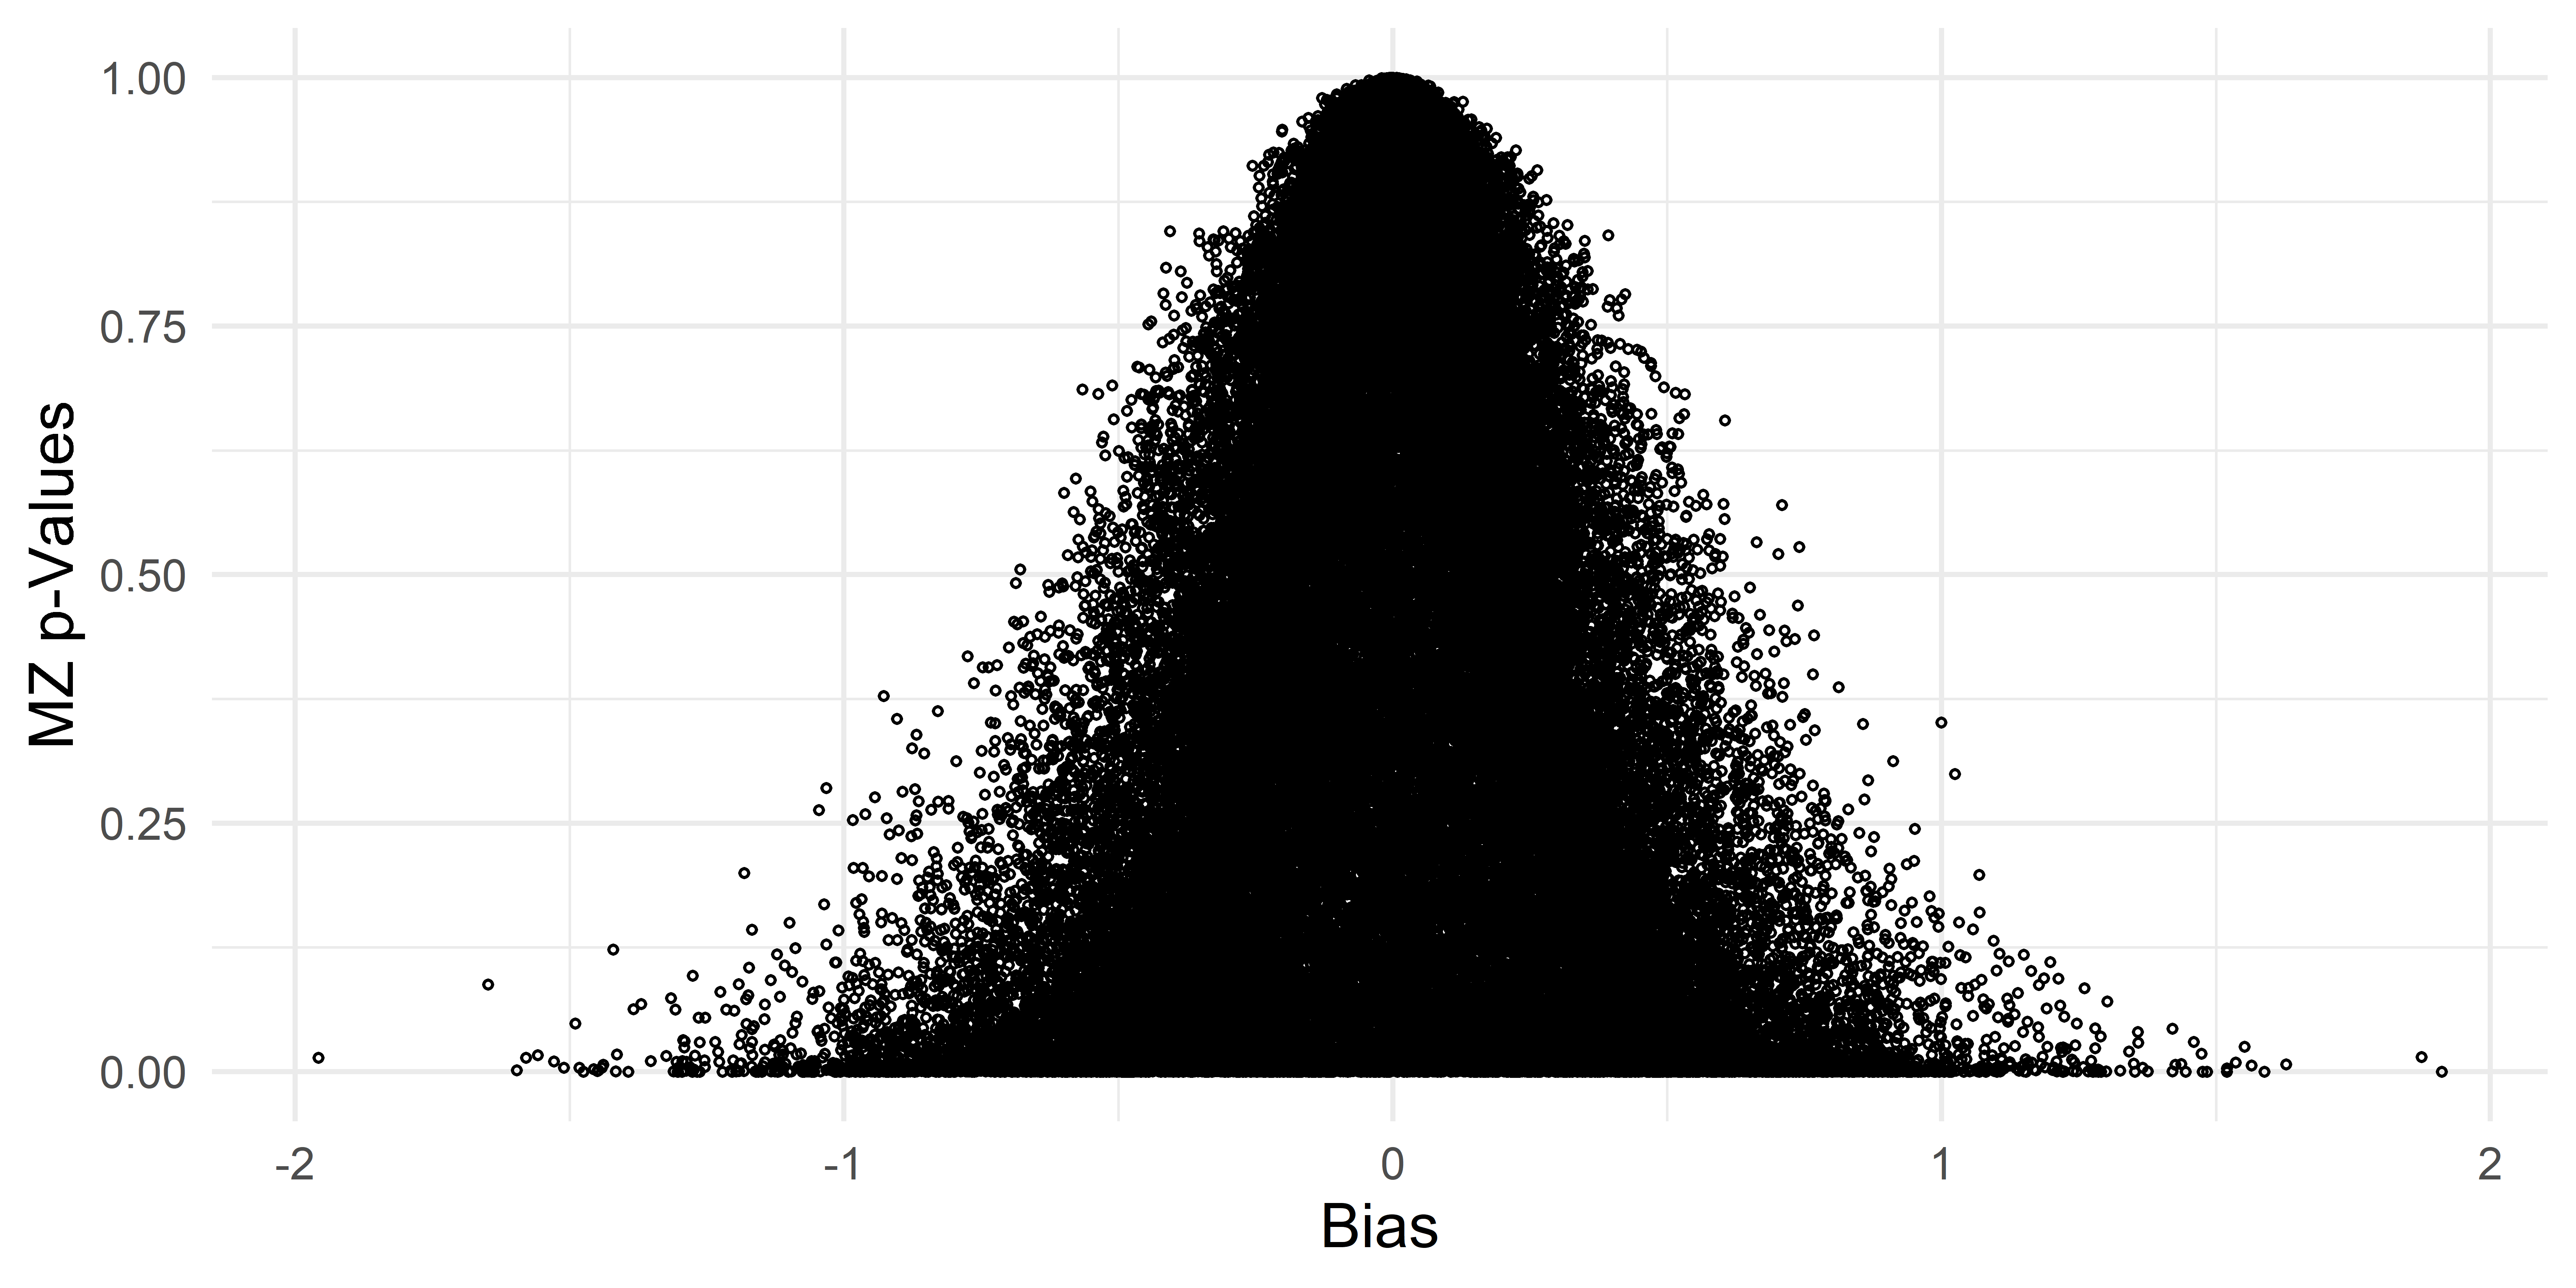
\includegraphics[scale=.9]{F09}
	\caption{\ac{MZ} p-values vs. respective bias for the REGSC-model}
	\label{F_08}
\end{figure}

\subsubsection{Summary}

\subsection{Dynamic Data Generating Processes}